\subsection{Recommended Build Directory Structure}
\label{subsect:BuildDirectoryStructure}

Via Autoconf and Automake the Trilinos configuration facilities
provide a great deal of flexibility for configuring and building the
existing Trilinos packages.  However, unless a user has prior experience
with Autotools, we very strongly recommend the following process to build and
maintain local builds of Trilinos.

To start, we defined two useful terms:
\begin{itemize}
\item Source tree - The directory structure where source files are found.  A source 
tree is obtained by expanding a distribution tar ball, or by checking 
out a copy of the Trilinos repository.  
\item Build tree - The directory structure where object and library files, as 
well as executables are located.  
\end{itemize}
 
\begin{minipage}[c]{\textwidth}

\begin{minipage}[l]{.6\textwidth}

Although it is possible to run \InlineCommand{./configure} from the source tree (in 
the directory where the configure file is located), we recommend 
separate build trees.  The greatest advantage to having a separate 
build tree is that multiple builds of the libraries can be maintained
from the same source tree.  For example, both serial and parallel libraries
can be built.  
This approach also eliminates problems with configuring in a 'dirty'
directory (one that has already been configured in).
\end{minipage}\hfill
\framebox{\begin{minipage}[r]{.35\textwidth}{
{\bf Key Point:}
$\ldots$ we recommend 
separate build trees $\ldots$ multiple builds of the
libraries can be maintained from the same source tree $\ldots$ 
problems with configuring in a 'dirty' directory (are eliminated) $\ldots$
}\end{minipage}}
\end{minipage}

Setting up a build tree is straight-forward.
Figure~\ref{Figure:TrilinosDirectoryStructure} illustrates the
\begin{figure}
\begin{center}
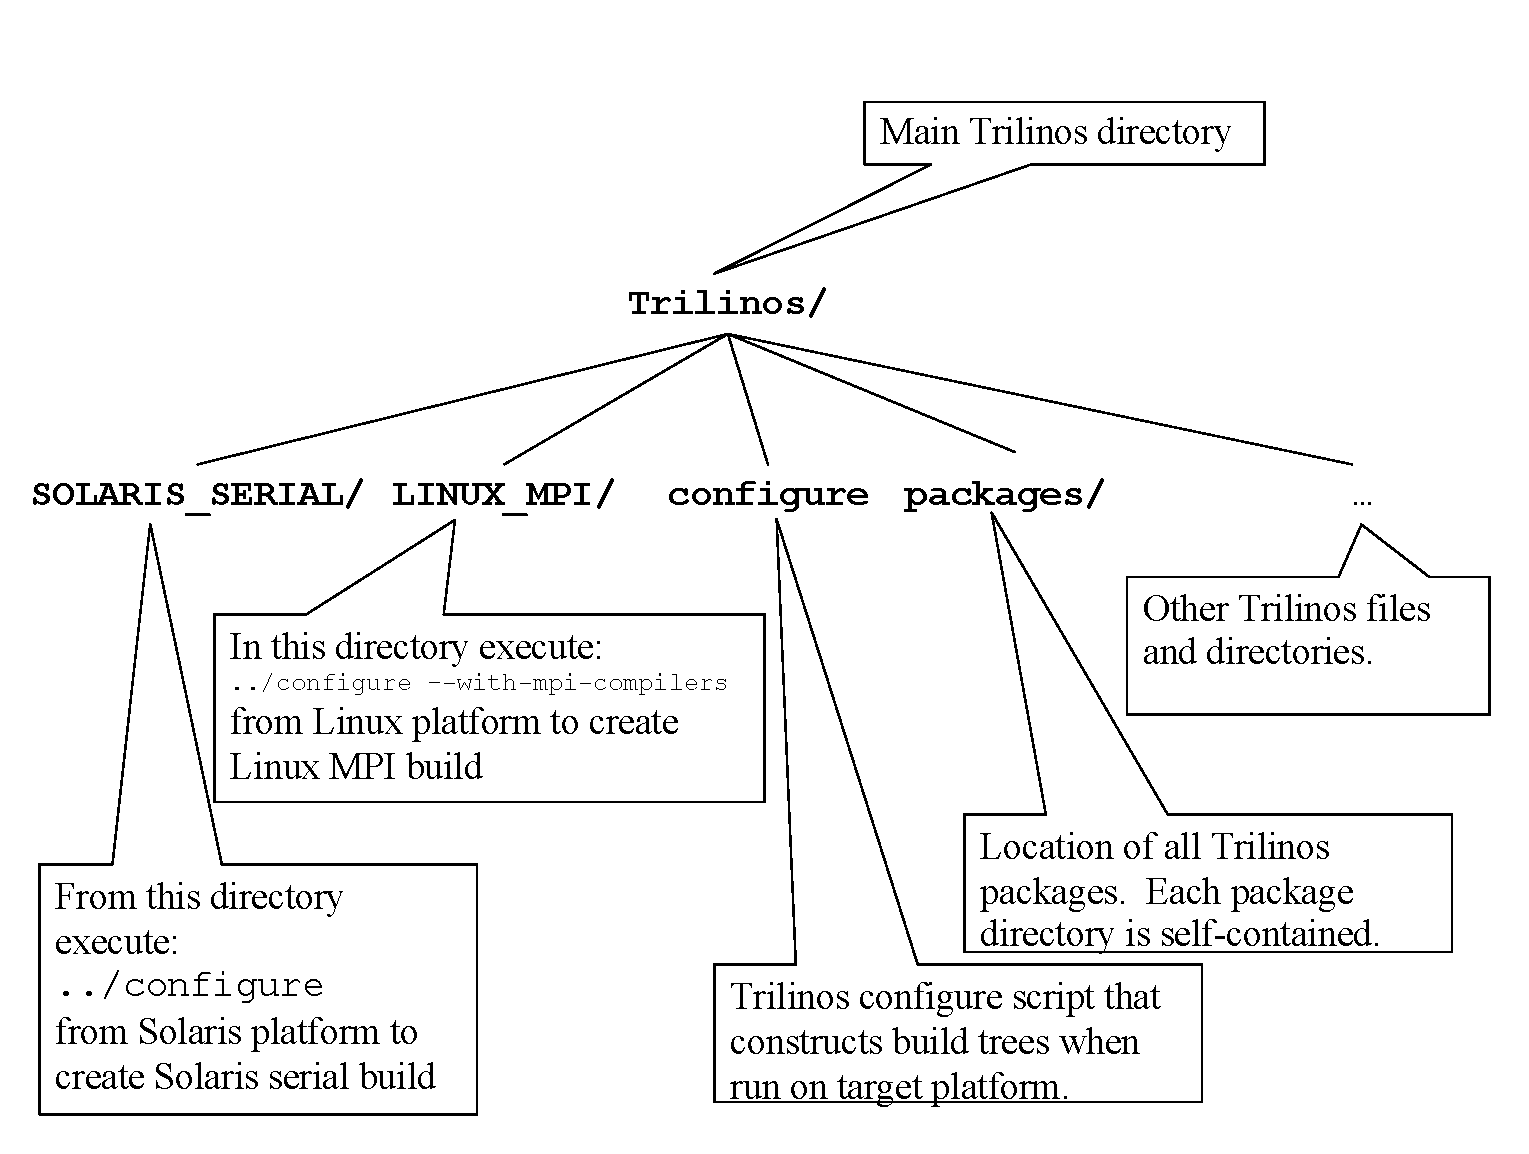
\includegraphics[width=6in]{../CommonFiles/TrilinosDirectoryStructure}
\end{center}
\caption{\label{Figure:TrilinosDirectoryStructure}Recommended Layout for Trilinos Build Directories}
\end{figure}recommended layout.  First, from the highest 
directory in the source tree (Trilinos for a repository copy, Trilinos-3.0.2 
for a distribution), make a new directory - for an MPI build
on a Linux platform, a 
typical name is \InlineDirectory{LINUX\_MPI}.  
Finally, from the new directory, type

\DisplayCommand{../configure --with-mpi-compilers}

(Note that various configure options might be necessary, see Section~\ref{Subsection:ConfiguringTrilinos} for details.)  Finally, type

\DisplayCommand{make}


In summary:

\begin{verbatim}
       cd Trilinos
       mkdir LINUX_MPI
       cd LINUX_MPI
       ../configure --with-mpi-compilers
       make
\end{verbatim}
At this point, the MPI version of Trilinos on a Linux platform is
built and completely contained in the \InlineDirectory{LINUX\_MPI}
directory.  No files outside this directory have been modified.  This
procedure can be repeated for any number of build targets.

{\bf Note:} Although we recommend the above location for build trees,
they can be set up anywhere.

\subsection{Configuring Trilinos}
\label{Subsection:ConfiguringTrilinos}

\begin{minipage}[c]{\textwidth}

\begin{minipage}[l]{.6\textwidth}

The most common issue encountered when configuring Trilinos is that it is 
nearly impossible to determine what caused configure to fail based on the 
standard output.  If the output from configure is inadequate, 
look at the config.log file (in the buildtree)
for the package that failed to configure properly.  

\end{minipage}\hfill
\framebox{\begin{minipage}[r]{.35\textwidth}{
{\bf Key Point:}
$\ldots$ to determine what caused configure to fail $\ldots$ 
look at the config.log file $\ldots$
}\end{minipage}}
\end{minipage}

To determine which 
package failed to configure, look at the bottom of the output from the 
\InlineCommand{configure} command.  One of the last lines will say something 
like:

\begin{verbatim}
    configure: error: /bin/sh '../../../packages/epetra/configure'
    failed for packages/epetra
\end{verbatim}

This particular error indicates to look in 
\InlineDirectory{packages/epetra/config.log}.

	To configure from a remote build tree, simply run the configure script 
in source tree from the root of the build tree.  In the example above, cd to 
the SOLARIS\_SERIAL directory and type 
\DisplayCommand{../configure <configure options>}

A detailed list of configure options can be seen by typing
\DisplayCommand{./configure --help=recursive} from the top level of the 
source tree.  This will display the help page for the Trilinos level as well as all 
Trilinos packages that use Autoconf and Automake.  The output from this command
is quite extensive.  To view the help page for an individual package, cd to 
the home directory for the package in the source tree and type 
\DisplayCommand{./configure --help} 
This command will also display the help page for Trilinos level 
options when used from the Trilinos home directory in the source tree.


Many of the Trilinos configure options are used to describe the details of the 
build.  For 
instance, serial or mpi, all of the packages, or just a proper subset.  

To configure for serial libraries, no action is necessary,
but to configure for parallel libraries, a user must append appropriate 
arguments to the configure invocation line as described in ``Trilinos 
Configuration Options'', section~\ref{subsect:TrilinosConfigOptions}.

Also, to build the default set of Trilinos libraries, no action is 
necessary, but to exclude a package that is built by default, AztecOO for 
example, append \newline \InlineCommand{--disable-aztecoo} to the configure 
invocation  line.  Similarly, to include a package that is not currently built 
by default, Komplex for example, append \InlineCommand{--enable-komplex} to 
the configure invocation line.  

\begin{minipage}[c]{\textwidth}
\begin{minipage}[l]{.6\textwidth}

Users are strongly encouraged to build 
only the packages that are necessary because configuring and 
building can take a long time.  It is well worth the time to look at which
packages are build by default enable and disable packages as necessary.
\end{minipage}\hfill
\framebox{\begin{minipage}[r]{.35\textwidth}{
{\bf Key Point:}
$\ldots$ build only the packages that are necessary because configuring and 
building can take a long time.
}\end{minipage}}
\end{minipage}

It is recommended that users always configure 
from the Trilinos level and use \InlineCommand{--disable-<package>} as 
required, rather than trying to configure from a lower level.  To see which 
packages are built by default and which ones aren't, simply cd to the Trilinos home directory and type \DisplayCommand{./configure --help}


{\bf NOTES:} 
\begin{enumerate}
\item {\bf Enabling/Disabling package builds:} 
The configure process is set up to detect when a 
\InlineCommand{--disable-<package>} option would break a package dependency.  
For example, Ifpack depends on Epetra, so if a user wants to build Ifpack, but 
types \InlineCommand{--disable-epetra}, Epetra will be configured and built 
anyway.  

\item {\bf Installing libraries and header files:}
To install libraries and header files in a particular location, 
use \InlineCommand{--prefix=<dir>} on the configure line.  If this option is 
used, libraries will be located in \InlineDirectory{<dir>/lib} and header files in 
\InlineDirectory{<dir>/include/<package>}.

\item {\bf Providing additional information to Autotools:}
Although Autotools will try to determine all configuration
information, the user must provide anything that Autotools needs and 
cannot find.  Also, if Autotools selects, for example, the wrong 
BLAS library by default, the user must indicate which BLAS library to use.  
Other issues such as standards 
non-compliance are also commonly dealt with using configure options.  
If all required libraries (often 
the BLAS and LAPACK) are located in standard places and no special 
compiler flags are required, try configuring without
providing additional information.

\item {\bf Sample configure invocation scripts:}

\begin{minipage}[c]{\textwidth}
\begin{minipage}[l]{.6\textwidth}

Sample configure invocation scripts for a wide variety of platforms can be 
found in \InlineDirectory{Trilinos/sampleScripts}.  These scripts are generally 
named using the following convention: \InlineCommand{arch\_comm\_machine}.
For example, \InlineCommand{sgi64\_mpi\_atlantis}.  
\end{minipage}\hfill
\framebox{\begin{minipage}[r]{.35\textwidth}{
{\bf Key Point:}
Sample configure invocation scripts for a wide variety of platforms can be 
found in \InlineDirectory{Trilinos/sampleScripts}.
}\end{minipage}}
\end{minipage}

Note that these scripts 
are examples only and are primarily useful for the values of options such as 
\InlineCommand{LDFLAGS}, \InlineCommand{CPPFLAGS}, 
and \InlineCommand{CXXFLAGS}.  Do not expect to be able to find a 
script that can be used without modification; try to find a script for a 
similar machine to use as a guide.  

The scripts in the 
repository are not always up to date.  If a user submits a script for a 
machine that few Trilinos developers have an account on, that script may 
become obsolete if it is not updated by the user who submitted it.

Users who create scripts for other machines are encouraged to check them into 
the repository for the benefit of other users.  Users who do not have access to
the repository can send scripts to trilinos-help@software.sandia.gov.

The following is an example configure invocation script for an SGI machine:

\begin{verbatim}
../configure --enable-mpi --with-mpi-libs=-lmpi \
--with-cflags=-64 --with-fflags=-64 \
--with-cxxflags="-64 -LANG:std  -LANG:ansi-for-init-scope=ON \
-ptused -DMPI_NO_CPPBIND" \
LDFLAGS=" -64 -L/usr/lib64/mips4/r10000 -L/usr/lib64/mips4 \
-L/usr/lib64 " \
--enable-epetraext --enable-new_package \
--disable-komplex --enable-tsfcoreutils
\end{verbatim}
\end{enumerate}

\subsection{Trilinos Configuration Options}
\label{subsect:TrilinosConfigOptions}
The following options apply to all Trilinos packages unless 
an option doesn't make sense for a particular package (for example, a 
package that does not include any Fortran code will not be sensitive to 
\InlineCommand{F77=g77}), or otherwise noted.  For options specific to 
an individual package, cd to the home directory of the 
package and type \DisplayCommand{./configure --help}

Basic Options

\begin{itemize}
\item \InlineCommand{--enable-examples}

Build examples for all Trilinos packages (that are sensitive to 
this option).  By default, this option is enabled.

\item \InlineCommand{--enable-tests} 

Build tests for all Trilinos packages (that are sensitive to this option).  
By default, this option is enabled.

\item \InlineCommand{--enable-debug} 

(NOX only.)  This turns on compiler debugger flags. It has 
not been fully tested. As an alternate, specify CXXFLAGS on the 
                 configure line.

\item \InlineCommand{--enable-opt}

(NOX only.)  This turns on compiler optimization flags. It 
has not been fully tested. As an alternate, specify CXXFLAGS on the 
                 configure line. 

\item \InlineCommand{--with-cppflags}

Specify additional preprocessor flags (e.g., "-Dflag -Idir") 

\item \InlineCommand{--with-cxxflags}

Specify additional C++ flags 

\item \InlineCommand{--with-ldflags}

Specify additional linker flags (e.g., "-Ldir") 

\item \InlineCommand{--with-ar}

Specify a special archiver command, the default is "ar cru". 
\end{itemize}

 Influential Environmental Variables

\begin{itemize}
\item \InlineCommand{CC}

C compiler command.

\item \InlineCommand{CFLAGS}

C compiler flags.

\item \InlineCommand{CXX}

C++ compiler command.

\item \InlineCommand{CXXFLAGS}

C++ compiler flags.

\item \InlineCommand{LDFLAGS}

Specify linker flags.

\item \InlineCommand{CPPFLAGS}

C/C++ preprocessor flags.

\item \InlineCommand{CXXCPP}

C++ preprocessor.

\item \InlineCommand{F77}

Fortran 77 compiler command.

\item \InlineCommand{FFLAGS}

Fortran 77 compiler flags.
\end{itemize}

MPI-Related Options

\begin{itemize}
\item \InlineCommand{--enable-mpi}

Enables MPI mode. Defines HAVE\_MPI in the (Package)\_Config.h file. Will test 
for the ability to preprocess the MPI header file and may test ability to link 
with MPI.  This option is rarely necessary as many of the below options also 
turn MPI on.  

\item \InlineCommand{--with-mpi-compilers}

Sets CXX = mpicxx (or mpiCC if mpicxx not available), CC = mpicc and 
F77 = mpif77.  Automatically enables MPI mode.  To use compilers other than 
these, specify MPI locations with the below options.  If none of these options 
are necessary, use \InlineCommand{--enable-mpi} to enable MPI mode.  In this 
case, CXX, CC, and F77 have to be set if the correct compilers are 
not chosen by default.

\item \InlineCommand{--with-mpi=MPIROOT}

Specify the MPI root directory. Automatically enables MPI mode.  If this 
option is set, \InlineCommand{--with-mpi-incdir} and 
\InlineCommand{--with-mpi-libdir} should not be used.  
\InlineCommand{--with-mpi} is a shortcut for setting \newline
\InlineCommand{--with-mpi-libdir=MPIROOT/lib} 
and \newline \InlineCommand{--with-mpi-incdir=MPIROOT/include}.

\item \InlineCommand{--with-mpi-libdir=DIR}

Specify the MPI libraries location. Defaults to MPIROOT/lib if 
\InlineCommand{--with-mpi} is specified. If multiple directories must be 
specified, try \newline
\InlineCommand{--with-ldflags="-L<dir1> -L<dir2>"} instead. 

\item \InlineCommand{--with-mpi-libs="LIBS"} 

Specify the MPI libraries. Defaults to \InlineCommand{"-lmpi"}
 if either\InlineCommand{ --with-mpi} or 
\InlineCommand{--with-mpi-libdir} is specified.

\item \InlineCommand{--with-mpi-incdir=DIR}

Specify the MPI include files location. Defaults to \InlineDirectory{MPIROOT/include} if 
\InlineCommand{--with-mpi} is specified. If multiple directories  must be specified, try 
\newline
\InlineCommand{--with-cppflags="-I<dir1> -I<dir2>"} instead.
\end{itemize}

Developer-Related Options
\begin{itemize}
\item \InlineCommand{--enable-maintainer-mode}

Enable make rules and dependencies not useful (and sometimes confusing) to 
the casual installer.
\end{itemize}

\subsection{Building and Installing Trilinos}

If the configure stage completed successfully, just type \DisplayCommand{make}
 and then, if 
\InlineCommand{--prefix} was specified, \DisplayCommand{make install}

\begin{minipage}[c]{\textwidth}

\begin{minipage}[l]{.6\textwidth}

Note that any code that links to Trilinos libraries must define
\InlineCommand{HAVE\_CONFIG\_H}.
\end{minipage}\hfill
\framebox{\begin{minipage}[r]{.35\textwidth}{
{\bf Key Point:}
... any code that links to Trilinos libraries must define
\InlineCommand{HAVE\_CONFIG\_H}.
}\end{minipage}}
\end{minipage}

\subsection{Configure, Make and Install: Common Problems}

\begin{minipage}[c]{\textwidth}
                                                                                
\begin{minipage}[l]{.6\textwidth}
Provided below is a list of common problems associated with configuring,
building and installing Trilinos.  A more complete FAQ list may be found online at
\end{minipage}\hfill
\framebox{\begin{minipage}[r]{.35\textwidth}{
{\bf Key Point:}
A more complete FAQ list may be found online...
}\end{minipage}}
\end{minipage}

\InlineCommand{http://software.sandia.gov/Trilinos/faq.html}.

\begin{itemize}

\item Any code that links to Trilinos libraries must define
\InlineCommand{HAVE\_CONFIG\_H}.

\item Do not attempt to specify optimization flags using the
\InlineCommand{--with-cxxflags}, \InlineCommand{--with-cflags}, or
\InlineCommand{--with-fflags} options.   Use \InlineCommand{CXXFLAGS},
\InlineCommand{CFLAGS} and \InlineCommand{FFLAGS} instead.  Use
\InlineCommand{--with-cxxflags}, \InlineCommand{--with-cflags}, and
\InlineCommand{--with-fflags} to specify flags that are to be used in
addition to the default optimization flags.
                                                                                
\item When creating a configure invocation script, be sure to use
line continuation characters properly.  The characters should be at the
end of every line, except the last line, and should not be followed by any
spaces.
                                                                                
\item To verify that the entire configure invocation script has been parsed by
Autoconf, open the \InlineDirectory{config.status} file in the top level of
the build tree and grep for the string "with options".  Here you will find all
of the options that Autoconf pulled from the invoke configure script.
                                                                                
\item Autoconf cannot detect most
spelling mistakes in configure invocation scripts.

\item When experiencing problems during the make phase, it is often useful to
\InlineCommand{make clean} before attempting to \InlineCommand{make} again.
Sometimes it even helps to blow away the entire build tree and start over.
                                                                                
\item When building with LAM under RH9 Linux, configure complains that it
cannot find mpi++.h.  The message in the config.log file is:
\begin{verbatim}
/usr/include/mpi.h:1064:19: mpi++.h: No such file or directory
\end{verbatim}
The following modified configure invocation works:
\DisplayCommand{../configure --enable-mpi CXX="mpiCC -DLAM\_BUILDING"}
                                                                                
\item The build process will fail on OSX if ``DropZip'' is used to
unzip the Trilinos tarball.  This utility truncates long file names.

\end{itemize}

\subsection{Tips for Making the Configure, Make, and Install Processes More Efficient}

Trilinos has grown to become a large piece of software.  Not surprisingly,
it can take a very long time to configure and build all of Trilinos.  Below 
are some tips for speeding up the process:

\begin{itemize}
\item Only build the Trilinos libraries that are necessary.

An easy way to do this is to use the --disable-default-packages option.  
This option allows users to easily specify exactly which packages should be 
built.  Packages that enabled 
packages are dependent on will be turned on automatically, so
don't shy away from disabling all packages that are not used directly.  
If a package configures and builds that was not enabled explicitly, 
keep in mind that a package that was enabled probably depends on that package.

\item Consider disabling tests and examples.

The first time Trilinos is built on a machine, it is a good idea to build 
and run some tests and examples.  After that, disabling tests and examples
can be considered as a way to speed up the build process.  To disable 
the tests and examples for all packages, use the 
\DisplayCommand{--disable-tests}

and

\DisplayCommand{--disable-examples}

options.  The speedup realized by disabling tests and examples will vary based 
on which packages are enabled; however, a speedup of about 1.6 could be 
expected for a ``typical'' mix of packages.

\item Cache configure results.

Adding 
\InlineCommand{--cache-file=config.cache}
to the list of configure arguments will store the results of many of the tests
that configure performs in a file called \InlineCommand{config.cache}, 
located in the top level of the build tree.

Using this option will allow the first package that is configured to store 
many test results that can be used by all subsequent packages.  If it is 
later necessary to reconfigure with a different set of packages, all packages
(including the first) can use these cached values.  If configure options are
changed that are associated with configure test results that have already 
been cached, or a relevant environment variable is changed, it is necessary 
to remove the
\InlineCommand{config.cache} file before reconfiguring.  Failing to do so
can cause the changes to be ignored.  

When configuring even a handful of 
packages, during the first configure a speedup of greater
than two is attainable and a speedup of greater than three is possible for 
subsequent configures.

\item Decrease build time on some machines by creating multiple jobs.

If \InlineCommand{-j} (jobs) is a valid option for \InlineCommand{make},
specifing the \InlineCommand{-j} option with a value of two times the number 
of processors that the machine has will typically result in a faster build 
process.  For example, on a dual processor machine, try replacing 
\InlineCommand{make} with 

\DisplayCommand{make -j 4}

during the build step.

On a single processor machine, the speedup is minimal; on a machine with 
multiple processors, the speedup can be quite significant.  For example, 
speedups of 1.73 and 2.45 were observed on a dual processor machine and a four 
processor machine, respectively.  Using two times the number of processors for 
the argument to the jobs option is only a suggestion based on observed 
performance; those who are interested in achieving optimal performance are
encouraged to experiment with various values and to report 
their findings to \InlineCommand{trilinos-help@software.sandia.gov}.  The 
\InlineCommand{-j} can also be passed without a corresponding value, in other 
words

\DisplayCommand{make -j}

When used in this way, the number of jobs created is unlimited.  For machines 
with a large number of processors this appears to work in some situations, but
machines with fewer than four processors tend to get bogged down with 
overhead.

\end{itemize}

